\documentclass{standalone}

\usepackage{tikz}
\usepackage{pgfplots}
\usepgfplotslibrary{groupplots}

\pgfplotsset{compat=1.18}

\begin{document}

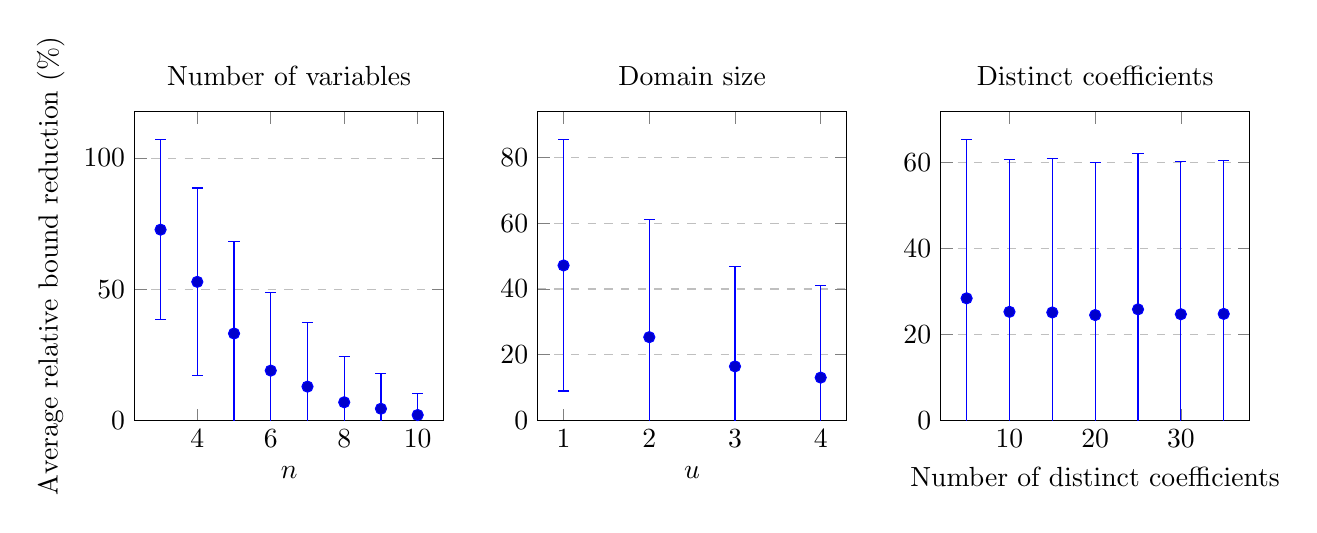
\begin{tikzpicture}

\begin{groupplot}[
    group style={
        group size=3 by 1,
        horizontal sep=1.2cm,
    },
    width=5.5cm,
    height=5.5cm,
    ymin=0,
    ymajorgrids=true,
    grid style={dashed},
]

% --------------------------------------------------
% Number of variables
% --------------------------------------------------

\nextgroupplot[
    title={Number of variables},
    xlabel={$n$},
    ylabel={Average relative bound reduction (\%)},
]

\addplot+[
    only marks,
    mark=*,
    error bars/.cd,
        y dir=both,
        y explicit,
]
coordinates {
    (3, 72.706912) +- (0, 34.227339)
    (4, 52.808403) +- (0, 35.787088)
    (5, 33.114542) +- (0, 35.002708)
    (6, 18.970441) +- (0, 29.707980)
    (7, 12.860745) +- (0, 24.518293)
    (8, 6.899346) +- (0, 17.585309)
    (9, 4.428422) +- (0, 13.463907)
    (10, 2.041778) +- (0, 8.334246)
};


% --------------------------------------------------
% Domain upper bound
% --------------------------------------------------

\nextgroupplot[
    title={Domain size},
    xlabel={$u$},
]

\addplot+[
    only marks,
    mark=*,
    error bars/.cd,
        y dir=both,
        y explicit,
]
coordinates {
    (1, 47.157220) +- (0, 38.220258)
    (2, 25.324259) +- (0, 35.704965)
    (3, 16.419752) +- (0, 30.361974)
    (4, 13.014064) +- (0, 27.975779)
};


% --------------------------------------------------
% Number of distinct coefficients
% --------------------------------------------------

\nextgroupplot[
    title={Distinct coefficients},
    xlabel={Number of distinct coefficients},
]

\addplot+[
    only marks,
    mark=*,
    error bars/.cd,
        y dir=both,
        y explicit,
]
coordinates {
    (5, 28.362602) +- (0, 36.828779)
    (10, 25.226963) +- (0, 35.445800)
    (15, 25.079085) +- (0, 35.866099)
    (20, 24.471639) +- (0, 35.479778)
    (25, 25.800922) +- (0, 36.210115)
    (30, 24.663318) +- (0, 35.490838)
    (35, 24.747238) +- (0, 35.657534)
};

\end{groupplot}

\end{tikzpicture}

\end{document}
